\chapter{Combo Extension Board}

What can we combine from servo, signal and GPIO to have one board for cases where too many lines are not necessary ?

\section{Schematics}

\begin{figure}[htbp]
    \centering
    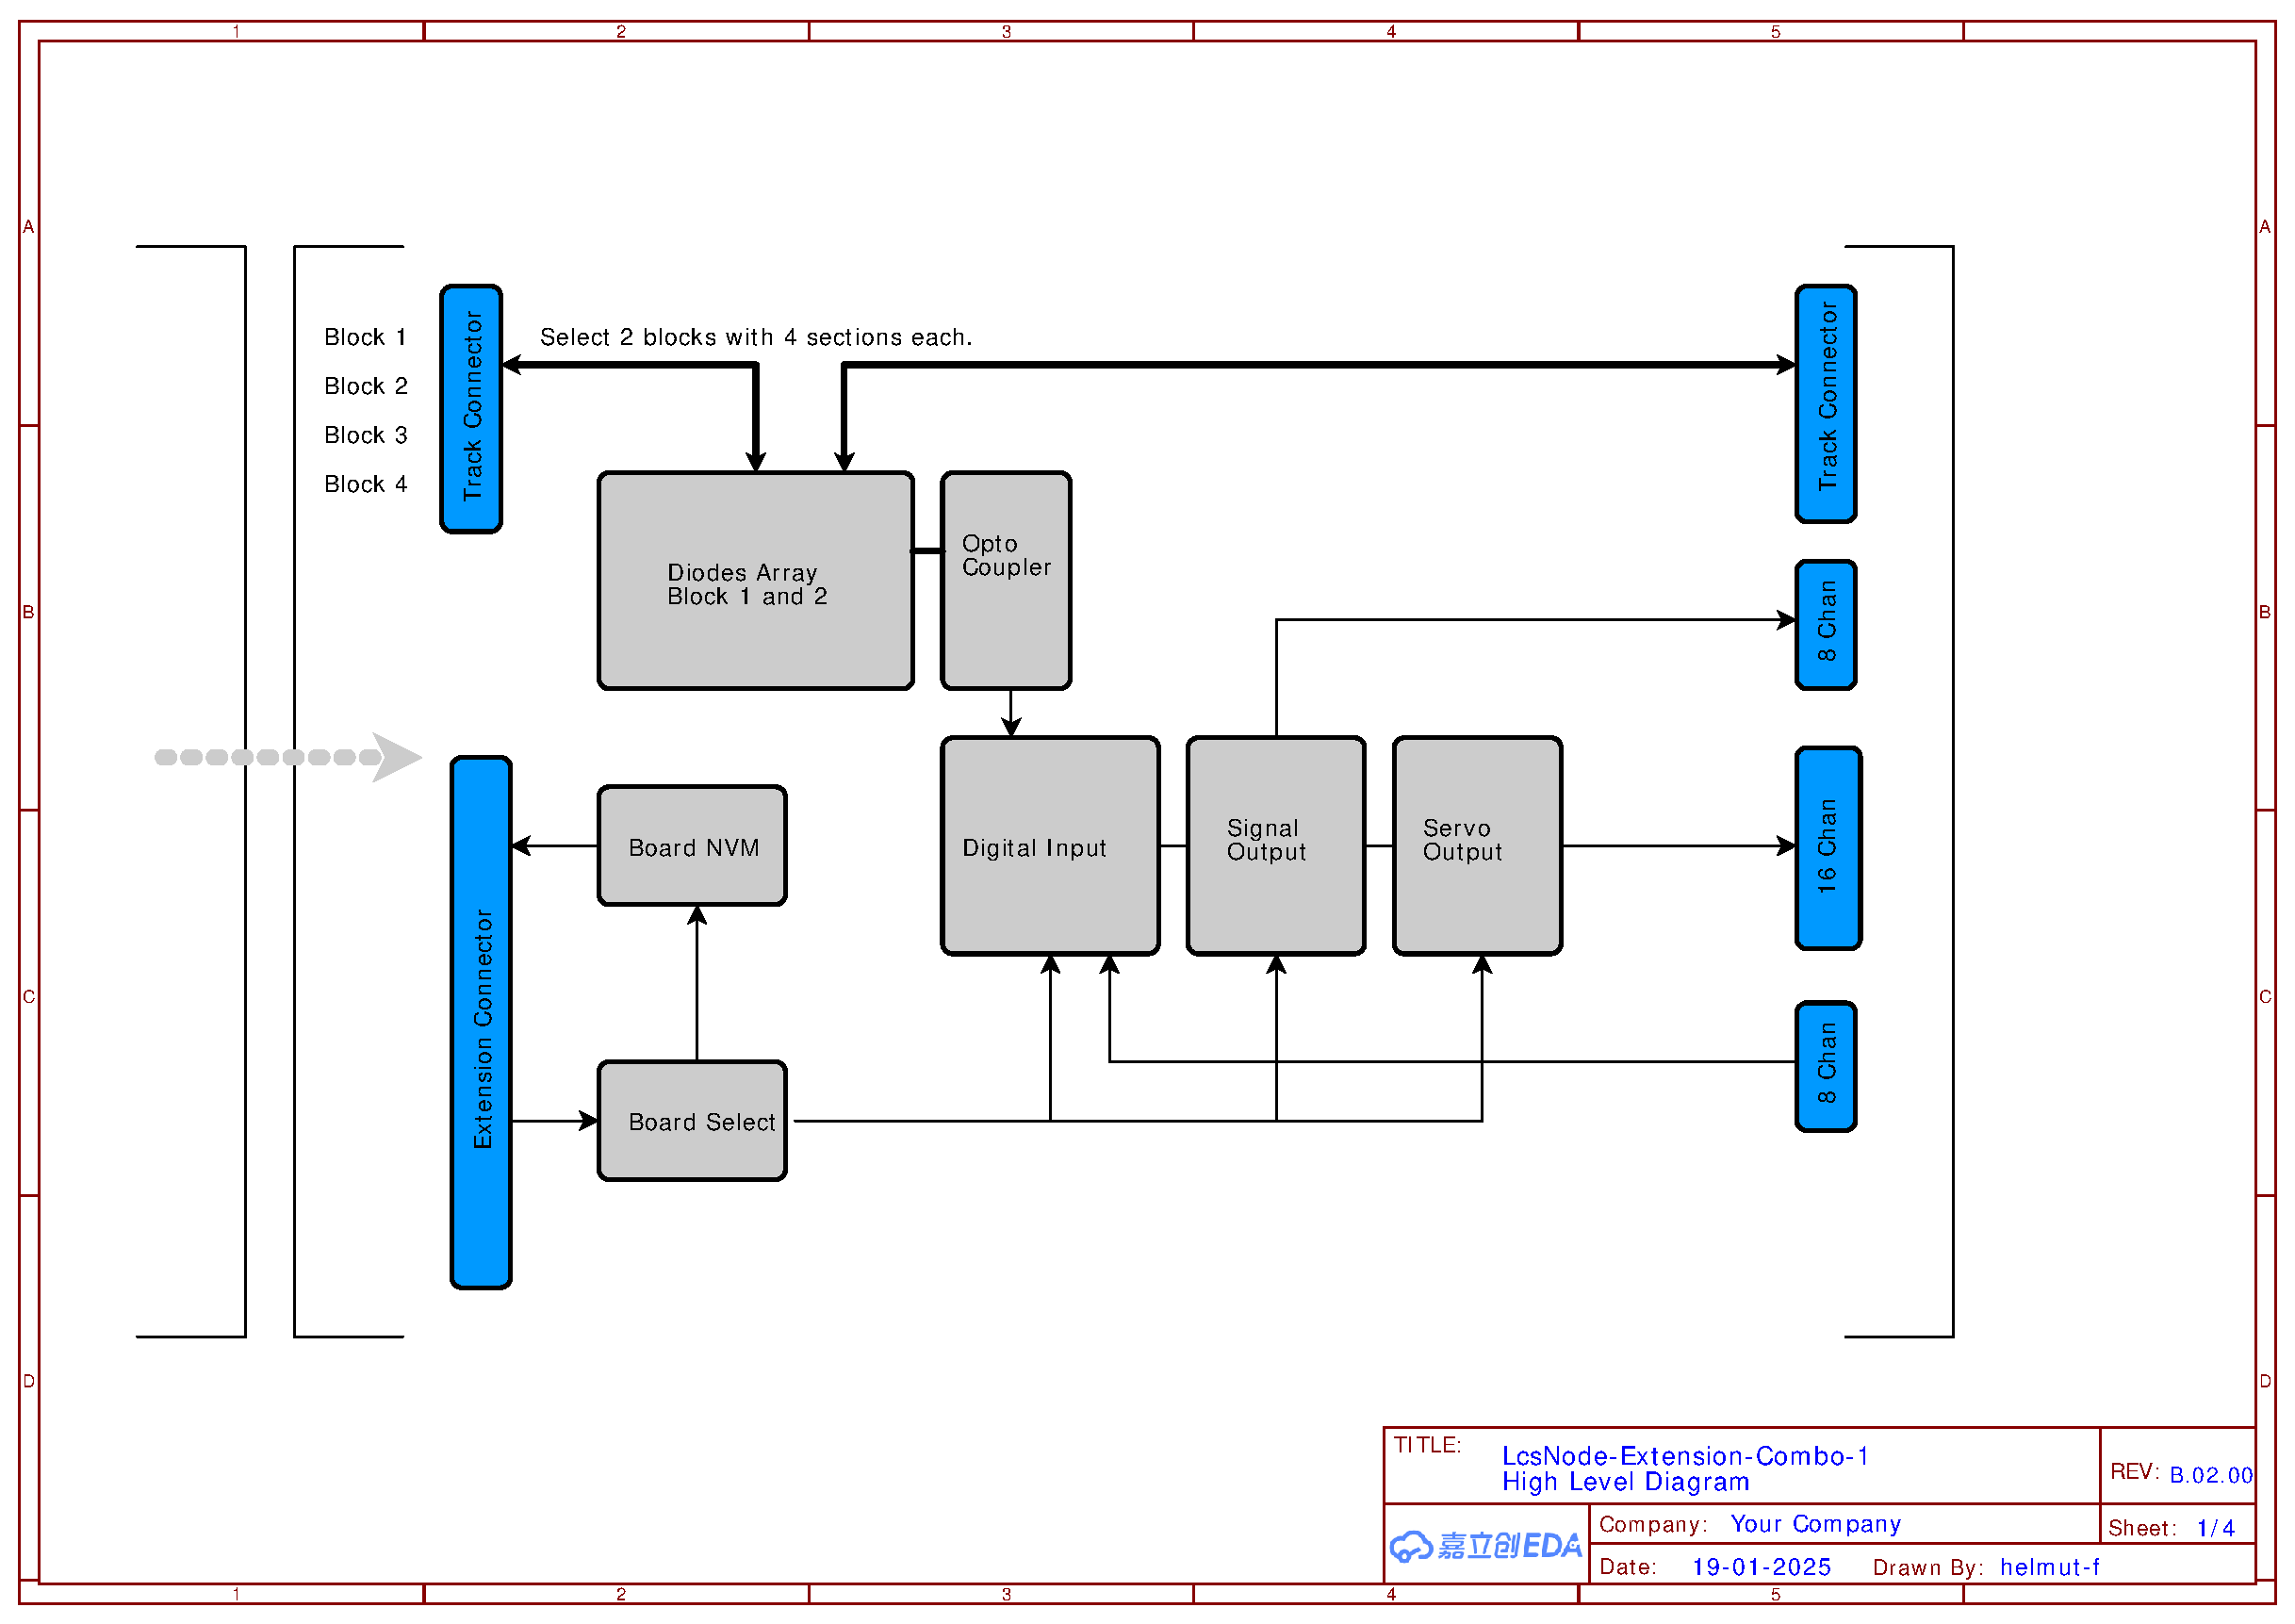
\includegraphics[page=1, width=0.7\textwidth]{./Schematics/Schematic_LcsNodes-Extension-Combo-1-Board.pdf}
    %\label{fig:schematic}
\end{figure}
\FloatBarrier

\begin{figure}[htbp]
    \centering
    \includegraphics[page=2, width=0.7\textwidth]{./Schematics/Schematic_LcsNodes-Extension-Combo-1-Board.pdf}
    %\label{fig:schematic}
\end{figure}
\FloatBarrier

\begin{figure}[htbp]
    \centering
    \includegraphics[page=3, width=0.7\textwidth]{./Schematics/Schematic_LcsNodes-Extension-Combo-1-Board.pdf}
    %\label{fig:schematic}
\end{figure}
\FloatBarrier

\begin{figure}[htbp]
    \centering
    \includegraphics[page=4, width=0.7\textwidth]{./Schematics/Schematic_LcsNodes-Extension-Combo-1-Board.pdf}
    %\label{fig:schematic}
\end{figure}
\FloatBarrier

\section{PCB}

\begin{tikzpicture}[scale=0.9, transform shape]

    \draw[help lines, gray!50, dashed] (0,0) grid( 16,8);
    \node at (8,4) {picture};

\end{tikzpicture}

\section{Firmware}

\section{Summary}
